\documentclass[dvisvgm,multi=true]{standalone}
\usepackage{mathmlcoresvg}
\begin{document}
%<figcaption><span>Figure 1: </span>Generic Box Model for MathML elements</figcaption>
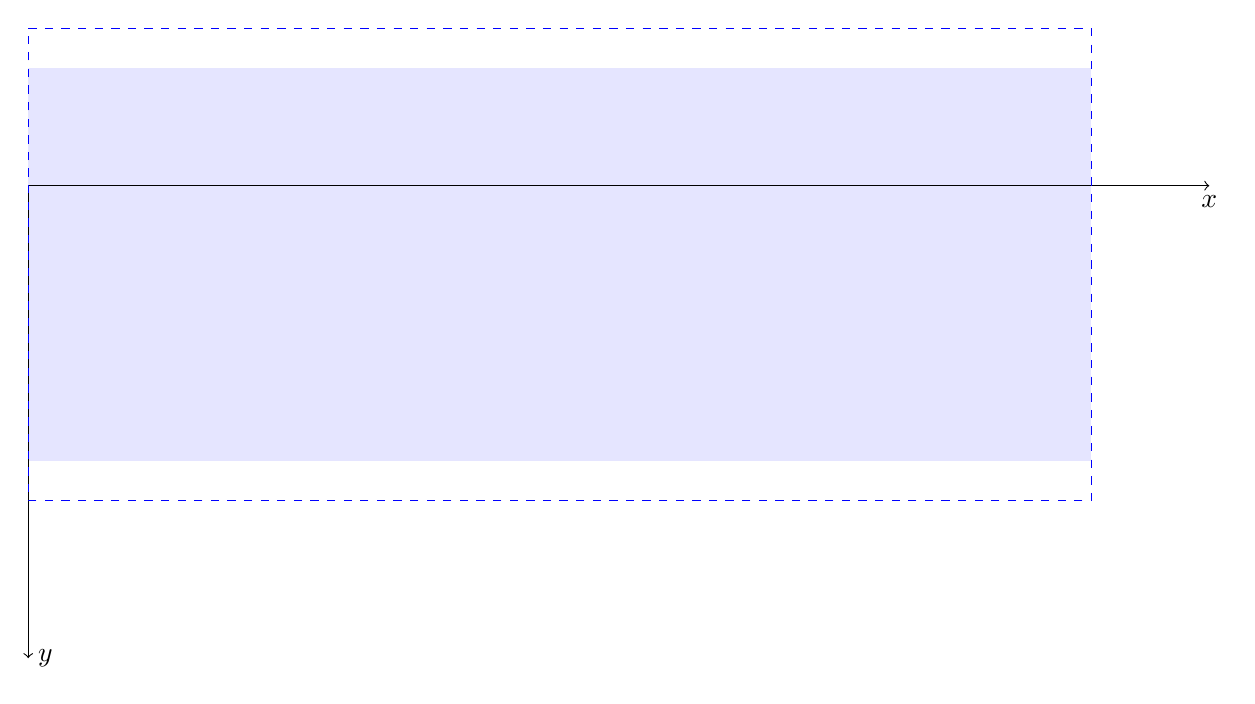
\begin{tikzpicture}[yscale=-1]
  \fill[blue!10] (0,-1.5) -- (13.5,-1.5) -- (13.5,3.5) -- (0,3.5) -- cycle;
  \draw[->] (0,0) -- (15,0) node[below] {$x$};
  \draw[->] (0,0) -- (0,6) node[right] {$y$};
  \draw[dashed,blue] (0,-2) -- (13.5,-2) -- (13.5,4) -- (0,4) -- cycle;
  \MathMLBox{0}{0}{1}{1}{red}
  \MathMLBoxMetrics{0}{0}{1}{1}{red}{1}
  \MathMLBox{6}{2}{1.5}{1}{green}
  \MathMLBoxMetrics{6}{2}{1.5}{1}{green}{2}
\end{tikzpicture}


\end{document}
